%----------------------------------------------------------------------------
\chapter{PSC – Property Sequence Charts}
%----------------------------------------------------------------------------
A Message Sequence Chart-nak nagyon sok hiányossága van.
Nem lehet vele megkötéseket definiálni vagy egy üzenetről eldönteni, hogy az egy elvárt vagy nem kívánt üzenet.
Ebből kifolyólag az MSC nem egy alkalmas nyelv arra, hogy az üzenet szekvenciáinkat részletesebben specifikálni tudjuk vele.

\begin{table}[ht]
    \centering % used for centering table
    \begin{tabular}{ |c|c|c| } % centered columns (4 columns)
    \hline
    \textbf{Tulajdonság} & \textbf{MSC} & \textbf{PSC} \\ [0.5ex] % inserts table
    %heading
    \hline % inserts single horizontal line
    \hline
    Nem kivánt üzenet & - & Fail message \\ % inserting body of the table
    \hline
    Elvárt üzenet & - & Required message \\
    \hline
    Sima üzenet & Default message & Regular message \\
    \hline
    Megkötött sorrendezés & - & Strict sequencing \\
    \hline
    Gyenge sorrendezés & Seq & Loose sequencing \\
    \hline
    Üzenet megkötések & - & Constraint \\
    \hline
    Alternatív lehetőségek & h-MSC & Alternative operator \\
    \hline
    Párhuzamos művelet & h-MSC & Parallel operator \\
    \hline
    Ciklus & h-MSC & Loop operator \\
    \hline %inserts single line
    \end{tabular}
    \label{table:nonlin} % is used to refer this table in the text
    \caption{Az MSC összehasonlítása a PSC-vel} % title of Table
\end{table}

A Property Sequence Chart[1] az MSC egy kiterjesztése.
Sok új elemet vezet be ami nincs az MSC-ben, melyek megtekinthetők a 2.1. táblázaton, mint az üzenet típusokat: sima üzenet (e), elvárt üzenet (r) és nem kívánt üzenet (f).
Így specifikálhatjuk, hogy mely üzenetek azok amik helyes viselkedésre utalnak és azok amelyek nem.
Az elvárt üzenetek azok az üzenetek amelyeknek feltétetlen meg kell történiük a rendszer működése során.
Egy sima üzenet nem jelent hibát a monitor szempontjából ha nem történik meg, viszont ha megjelenik, akkor a scenario-ban utána következő üzenetek ellenőrzésére kell áttérni.
Szigorú sorrendezésre is ad megoldást a PSC, ami azt jelenti, hogy megadhatjuk explicit az üzenetek sorrendjét a követelményünkben.
A PSC-ben egy üzenetre megkötést is rakhatunk.
Megadhatjuk, hogy melyek azok az üzenetek amik nem kívántak az üzenetünk előtt vagy után.
A különböző PSC tulajdonságok megtalálhatok a 2.1. ábrán.
A nyelv a következő tulajdonságokat támogatja:

\begin{itemize}
    \item \textit{Sima üzenet (e)}: egy üzenet a scenario-ban, amely ha nem történik meg az a monitor szempontjából nem jelent hibát.
    Viszont ha megjelenik, akkor a scenario-ban utána következő üzenetek ellenőrzésére kell áttérni.
    Egy előfeltételt reprezentál.
    \item \textit{Elvárt üzenet (r)}: egy üzenet amelynek elmaradása hibajelzéshez kell vezessen.
    \item \textit{Nem kívánt üzenet (f)}: amennyiben a monitor egy ilyen üzenetet detektál, akkor hibát jelez.
    \item \textit{Üzenet megkötés (constraint)}: Egy üzenetre lehet megkötést is helyezni.
    Egy megkötés több üzenetet tartalmazhat.
    Két fajta megkötést definiál a nyelv: múlt- és jövőbéli.
    A múltbéli üzenet megkötés esetén, az üzenetünk megtörténte előtt, a megkötésben szereplő üzenetek egyike se történhet meg.
    Jövőbéli megkötés esetén, pedig az üzenetünk megtörténte után nem történhetnek meg a megkötésben szereplő üzenetek.
    \item \textit{Megkötött sorrendezés (strict ordering)}: A PSC az üzenet lefutási sorrendjének a specifikálására is lehetőséget ad.
    Egy „a” üzenet megtörténte után, egy adott „b” üzenetnek kell bekövetkeznie.
    Ha „b” üzenet helyet egy másik üzenet követi az „a” üzenetet, akkor a monitor hibát jelez.
\end{itemize}

A nyelv támogat összetett szerkezeteket is:

\begin{itemize}
    \item \textit{Alt operátor}: az alt operátorral alternatív üzenet szekvenciákat lehet definiálni.
    \item \textit{Par operátor}: a par operátorral meghatározható az üzenet szekvenciák párhuzamos futása.
    \item \textit{Loop operátor}: a loop operátorral megadhatjuk, hogy egy üzenet szekvencia többször is lefuthat egymás után.
\end{itemize}

Egy üzeneten egyszerre megkötés és sorrendezés is lehet.
Az üzenetek típusát az átmenetén lévő karakterrel jelöljük.
Az „e” karakter jelzi, hogy az üzenet sima, az „r” karakter az elvárt üzenetet jelenti, az „f” pedig a nem kívánt üzenetet.
Azt meg kell jegyezni, hogy nem kívánt üzenetekre nem lehet jövőbéli megkötéseket rakni.
Ezen kívül, ha egy üzeneten megkötött sorrendezést alkalmazunk, akkor nem lehet rajta múltbéli megkötés.

A megkötéseket egy ponttal jelöljük, amit az átmeneten helyezünk el.
Ha a pont az átmenet elején van (a feladóhoz közel), akkor az múltbéli megkötést jelöl.
Ha pedig a végén helyezkedik el, akkor a jövőbéli megkötést jelöli.
A megkötésben lévő üzeneteket egy lista formájába lehet megadni ’{’ ’}’ jelek közt, a következő módon: <megkötés neve> = {C1.I1.Cj, ..., Ck.In.Ct}, ahol az üzenetek vesszővel elválasztva, „Feladó.Üzenet.Címzett” formában szerepelnek.
A specifikált megkötés nevét pedig az átmeneten lévő pont alá írjuk.

Az üzenetek megkötött sorrendezésének jelölésénél az objektum „life line” vonalát az érintett átmenetek közt folytonossá változtatjuk

\begin{figure}[!ht]
    \centering
    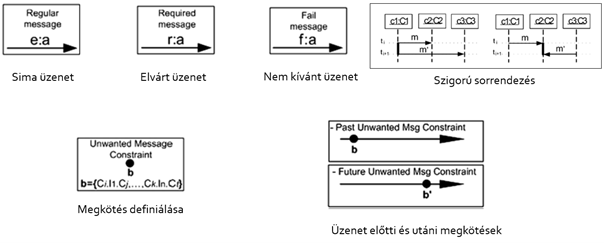
\includegraphics[width=150mm, keepaspectratio]{figures/2abra.png}
    \caption{A PSC különböző elemei[1].}
\end{figure}

Az üzeneteket a következő formában adjuk meg: \textit{Feladó.Üzenet.Címzett}.

\begin{figure}[!ht]
    \centering
    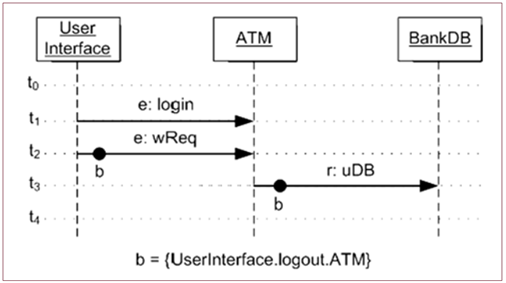
\includegraphics[width=130mm, keepaspectratio]{figures/3abra.png}
    \caption{PSC diagram egy ATM rendszer működésének ellenőrzésére[1].}
\end{figure}
A 2.2. ábrán láthatunk egy példát arra, hogy egy követelményt hogyan lehet definiálni.
Ez a PSC diagram egy ATM rendszer működését figyeli.
Először a felhasználó egy \textit{login} üzenettel bejelentkezik az ATM-be majd egy \textit{wReq} üzenettel egy lekérdezést hajt végre.
Ezen az üzeneten van egy megkötés, az üzenet előtt nem történthet kijelentkezés, \textit{logout}.
Az ATM ezután, ha nem történt \textit{logout} egy elvárt üzenetet küld a Bank adatbázisába.

A scenario-ink specifikálására most már rendelkezésünkre áll egy grafikus nyelv.
A következőkben az lesz a feladatunk, hogy ezeket a diagramokat úgy transzformáljunk, hogy monitor kódot lehessen belőlük készíteni.
